\section{Interpretácia výstupov modelov}

Jednou z najväčších výziev pri problematike predikcie bankrotu je jeho nízka prevalencia v populácii firiem.
Aj pri pohľade na iné krajiny je zrejmé, že počet firiem v bankrote každoročne predstavuje takmer vždy menej než 1 \% z celkovej populácie
firiem v krajine \cite{gruszczynski} (TODO: možno priamo nejaké OECD by som mohol zazdrojovať).
V reči pravdepodobnosti a štatistiky tento fenomén nazývame problémom nevyvážených tried (angl. \emph{imbalanced classes}).

V \cite{gruszczynski} autor definuje dva druhy nevyváženosti v dátach.
Majme vzorku \(n\) firiem, ktorá obsahuje \(n_1\) firiem v bankrote a \(n_2\) prosperujúcich firiem (prirodzene \(n_1 + n_2 = n\)).
Vzorku považujeme za nevyváženú, ak:

\bigskip
a) pomer \(n_1\) a \(n_2\) (firiem v bankrote a prosperujúcich firiem) vo vzorke je iný než \(50:50\), alebo

b) podiely \(p_1 = n_1/n\) a \(p_2 = n_2/n\) sú odlišené od podielov firiem v bankrote a prosperujúcich firiem v populácii.
\bigskip

Dôsledkami nevyváženosti dát pre problematiku predikcie bankrotu sa venujeme bližšie v tejto kapitole. (TODO: tu by sa hodila ešte jedna-dve vety o a) a b))

\subsection{„Biases“}

Modely predikcie bankrotu sa spravidla modelujú na nenáhodných vzorkách dát, čo má za následok  prítomnosť tzv. \emph{sample-choice bias}
(„zaujatosť“ modelu vznikajúcu následkom toho, že model vznikol práve na základe tej danej trénovacej sady dát, a nie inej).
Nenáhodnosť v dátach vzniká vtedy, keď zaradenie či nezaradenie danej firmy do trénovacej vzorky nie je skutočne náhodné, ale závisí od samotných hodnôt vysvetľovaných premenných
(napr. keď sa prosperujúce firmy vyberajú na základe podobnosti k firmám v bankrote) alebo je podmienené tým, že dáta pre danú firmu sú kompletné
(t.j. do trénovacej vzorky nezaraďujeme firmy, ku ktorým chýbajú niektoré údaje, čo v prípade finančných dát nie je výnimočný jav).

Z uvedeného vyplýva, že aj trénovacia vzorka, s ktorou sme pracovali v tejto práci, je v skutočnosti nenáhodná.
Spomeňme si, že firmy v bankrote sme do trénovacej vzorky (resp. do vzorky, z ktorej sme následne náhodne vybrali 80 \% dát) zaradili všetky (po očistení nehodiacich sa prvkov),
a prosperujúce firmy sme zvolili „párovacou“ metódou (angl. \emph{matched-pairs sample design}) na základe podobnosti odvetvia a tržieb.
Navyše, množina prosperujúcich firiem, v ktorej sme k firmám v bankrote hľadali pár, bola vopred zúžená len na firmy, pre ktoré sme mali k dispozícii kompletné dáta.
Rozdelenie firiem na trénovaciu a testovaciu vzorku v pomere \(80:20\) už bolo náhodné, ale to nemení nič na skutočnosti, že spojená množina trénovacích a testovacích dát vznikla deterministicky.

V problematike predikcie bankrotu avšak deterministickosť trénovacej vzorky nie je vôbec výnimočná;
podľa článku \cite{zmijewski} z roku 1984 až 70 \% článkov venujúcich sa bankrotu využíva na vytvorenie trénovacej sady práve párovaciu metódu, vrátane najznámejšej štúdie Altmana z roku 1968.
Párovacia metóda sa využila aj v niektorých novších článkov, viď napr. \cite{bodle}.

Jednou z výhod logistickej regresie (oproti napr. diskriminačnej analýze) je to, že pri predikcii má jej výstup jasnú interpretáciu –
predstavuje pravdepodobnosť, že daný pozorovaný objekt patrí do triedy \(Y = 1\).
Pri prítomnosti silnej nevyváženosti tried v populácii a nenáhodnosti trénovacej sady dát vyvstáva otázka, či sa táto interpretácia nestráca.

V práci sme vytvorili tri modely logistickej regresie, pričom vytvárali sme ich na základe trénovacej vzorke dát veľkosti \(1832\) firiem, kvalitu modelov sme vyhodnocovali na vzorke \(458\) firiem.
V oboch vzorkách bol pomer prosperujúcich firiem a firiem v bankrote \(50:50\).

\begin{figure}
    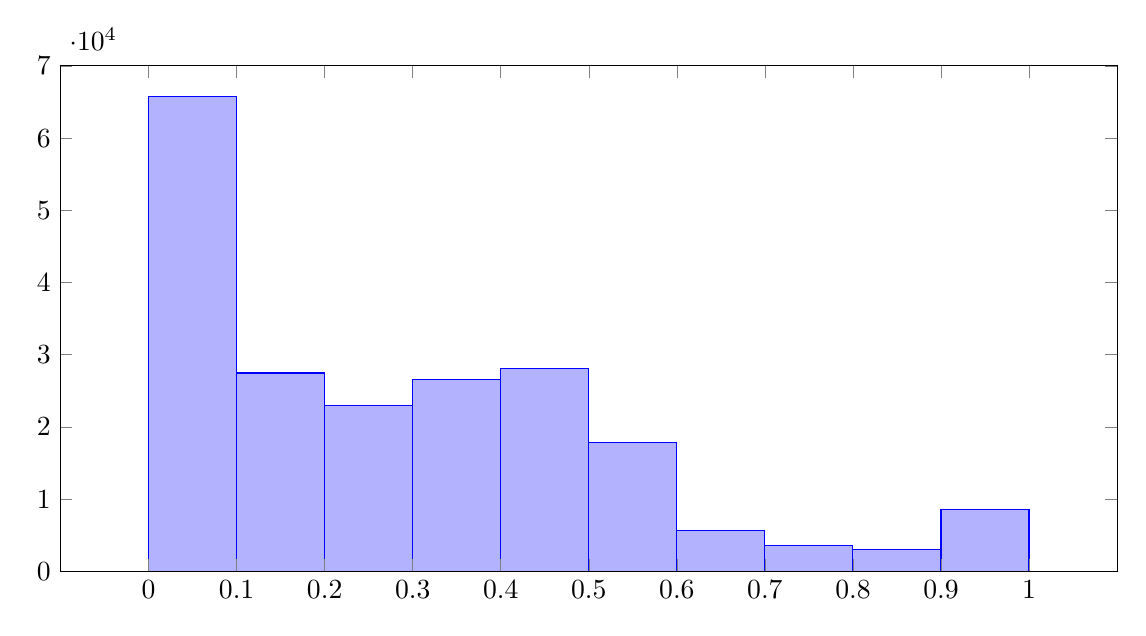
\begin{tikzpicture}
        \begin{axis}[
            ymin=0, ymax=70000,
            % minor y tick num = 2,
            area style,
            xtick={0,0.1,0.2,0.3,0.4,0.5,0.6,0.7,0.8,0.9,1},
            ytick={0,10000,20000,30000,40000,50000,60000,70000},
            style={
                /pgf/number format/fixed,
                /pgf/number format/precision=5
            },
            height=8cm,
            width=15cm,
            ]
        \addplot+[ybar interval,mark=no] plot coordinates {
            (0, 65752) (0.1, 27461) (0.2, 22984) (0.3, 26604) (0.4, 28083) (0.5, 17893) (0.6, 5689) (0.7, 3599) (0.8, 2979) (0.9, 8599) (1, 0)
        };
        \end{axis}
    \end{tikzpicture}
\caption{Histogram výstupov modelu BACE pre populáciu \(212169\) slovenských firiem}
\label{model_bace_whole_pop}
\end{figure}

Obrázok \ref{model_bace_whole_pop} predstavuje histogram výstupov modelu logistickej regresie \autoref{modely bace} (\emph{BACE} model kompletnej enumerácie)
v rámci celej populácie slovenských firiem s dostatočným množstvom dát na ich výpočet za rok 2019.
Z celkového počtu \(212169\) vypočítaných pravdepodobností \(40849\) vyšlo vyššie ako \(0.5\),
čo pri bežnom ponímaní logistickej regresie znamená, že \(40849\) firiem bolo zaradených do skupiny firiem v bankrote.

Obrázok \ref{altman_whole_pop} predstavuje histogram hodnôt Altmanovho \(Z\)-skóre na tej istej množine (pozn. histogram je očistený o extrémne hodnoty).
Podľa \(Z\)-skóre je firma v zóne bankrotu, ak \(Z > 2.9\), čo v rámci tejto množiny platí až pre \(90361\) firiem.
Ak by sme výstup logistickej regresie vyšší než \(0.5\), resp. výstup \(Z\)-skóre vyšší než \(2.9\), vnímali striktne ako prediktor (?) bankrotu,
pri nameranej senzitivite týchto modelov v rozmedzí 70-90 \% by to znamenalo, že v roku 2020 majú vyhlásiť bankrot rádovo desiatky tisíc firiem.

\begin{figure}
    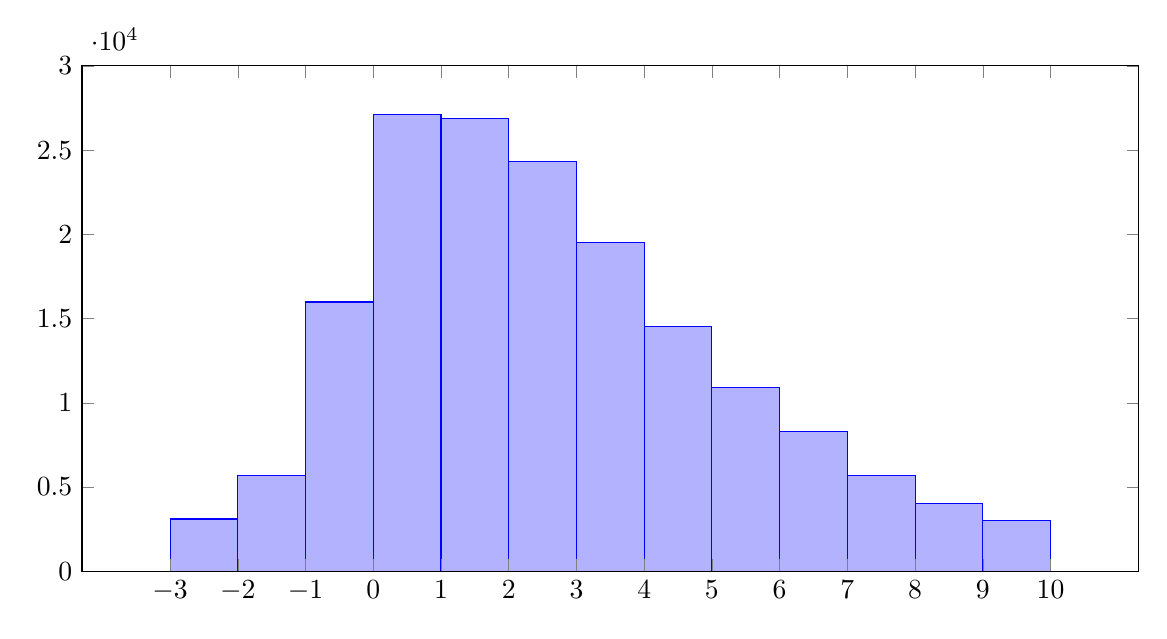
\begin{tikzpicture}
        \begin{axis}[
            ymin=0, ymax=30000,
            % minor y tick num = 2,
            area style,
            xtick={-3,-2,-1,0,1,2,3,4,5,6,7,8,9,10},
            ytick={0,5000,10000,15000,20000,25000,30000},
            yticklabel style={
              /pgf/number format/fixed,
            },
            % style={
            %     % /pgf/number format/fixed,
            %     /pgf/number format/precision=0,
            % },
            height=8cm,
            width=15cm,
            ]
        \addplot+[ybar interval,mark=no] plot coordinates {
            (-3, 3107) (-2, 5693) (-1, 15988) (0, 27101) (1, 26871) (2, 24310) (3, 19518) (4, 14516) (5, 10884) (6, 8295) (7, 5693) (8, 4007) (9, 2993) (10, 2320)
        };
        \end{axis}
\end{tikzpicture}
\caption{Histogram Altmanovho \(Z\)-skóre pre populáciu \(212169\) slovenských firiem (interval \((-3, 10)\))}
\label{altman_whole_pop}
\end{figure}

Takéto závery samozrejme nie sú správne. Skutočnosť, že modely predikcie bankrotu majú tendenciu prikláňať sa k triede firiem v bankrote,
vyplýva práve z nerovnakosti podielu firiem v bankrote v rámci trénovacej vzorky a celej populácie.
Možným vysvetlením tohto javu môže byť to, že trieda prosperujúcich firiem v trénovacej sade je málo reprezentovaná.
V prípade párovacej metódy sa prosperujúce firmy v trénovacej sade silno obmedzujú len na tie firmy, ktoré majú podobné vlastnosti firmám v bankrote,
z čoho zrejme vyplýva existencia veľkej množiny prosperujúcich firiem, ktoré v trénovacej sade nemajú reprezentanta ani zo svojho širšieho okolia (v zmysle podobnosti finančných ukazovateľov).
Navyše, je pravdepodobné, že práve táto nereprezentovaná skupina obsahuje mnoho firiem, ktoré by boli dobrým reprezentantom \emph{skutočne} prosperujúcich firiem
(prosperujúcich nielen v tom zmysle, že nikdy nevyhlásili bankrot ani reštrukturalizáciu, čo je definícia, ktorú sme zaviedli pre účely tejto práce).

Tendenciou bankrotných modelov prikláňať sa k triede firiem v bankrote sa zaoberal už Zmijewski v práci z roku 1984 \cite{zmijewski}, ktorú sme citovali už viackrát.

Pri zjavných limitáciách párovacej metódy pri výbere trénovacej sady dát vyvstáva otázka, či by nebolo vhodnejšie použiť iný prístup.
Rôznym metódam výberu trénovacej sady v problematike predikcie kreditného rizika sa zaoberá \cite{protopapadakis}.
Medzi metódami, ktoré v tejto práci autori porovnávajú, sa párovacia metóda síce nevyskytuje, práca ale zároveň nepreukázala významný prínos použitia sofistikovanejších techník výberu vzorky
(napr. rôznych kombinácií zhlukovacích algoritmov ako \(k\)-means či \emph{OPTICS}, spojených s náhodným výberom) oproti jednoduchému náhodnému výberu z množiny prosperujúcich firiem.
Zo záverov tejto práce, aj zo skutočnosti, že párovacia metóda predstavuje v rámci problematiky predikcie bankrotu „klasický prístup“, je zrejmé, že použitie párovacej metódy je adekvátne.

\subsection{Apriórna korekcia}

Jednou z metód na zmiernenie vplyvu nevyváženosti tried na model logistickej regresie je použitie tzv. apriórnej korekcie (angl. \emph{prior correction}).
Autorstvo apriórnej korekcie je diskutovanou témou, spomína sa vo viacerých prácach zo 70. rokov \cite{manski, bishop, anderson}.
Apriórna korekcia je v niektorých textoch známa aj ako Andersonova-Maddalova korekcia \cite{maddala}.

Majme model logistickej regresie s parametrom \(\beta = (\beta_0, \beta_1, \ldots, \beta_k) \) vytvorený na vzorke dát veľkosti \(n\),
pričom nech počet firiem v bankrote v rámci tejto vzorky je \(n_1\) a počet prosperujúcich firiem je \(n_2\).
Označme \( \bar{y} = n_1/n \) podiel firiem v bankrote v rámci trénovacej sady dát.
Podmienkou použitia apriórnej korekcie je poznanie skutočnej prevalencie firiem v bankrote v rámci celej populácie; túto prevalenciu označme \(\pi\).
V praxi nám stačí odhad hodnoty \(\pi\).
Keďže pri problematike bankrotu máme populáciu firiem dobre zdokumentovanú, predpokladajme, že predchádzajúca prevalencia firiem v bankrote je dostatočne dobrým odhadom hodnoty \(\pi\).

Apriórna korekcia spočíva v odpočítaní hodnoty delta od intereceptu \(beta_0\), pričom:

\[
    \delta = \ln \left[ \left( \frac{1 - \pi}{\pi} \right) \left( \frac{\bar{y}}{1 - \bar{y}} \right) \right].
\]

Uvedomme si, že v prípade náhodného výberu platí \( \bar{y} = \pi \), a teda \( \delta = 0 \).

Obrázok \ref{correction_demo} ilustruje vplyv korekcie pre hodnoty \( \pi = 0.01 \) a \( \bar{y} = 0.5 \) (trénovacia vzorka s pomeromo prosperujúcich firiem a firiem v bankrote \(50:50\)).
Upraveným pravdepodobnostiam modelu s korekciou napr. \(0,005, 0.01, 0.02, 0.10\) zodpovedajú výstupy pôvodného modelu \(0.33, 0.5, 0.67, 0.92\).

\begin{figure}
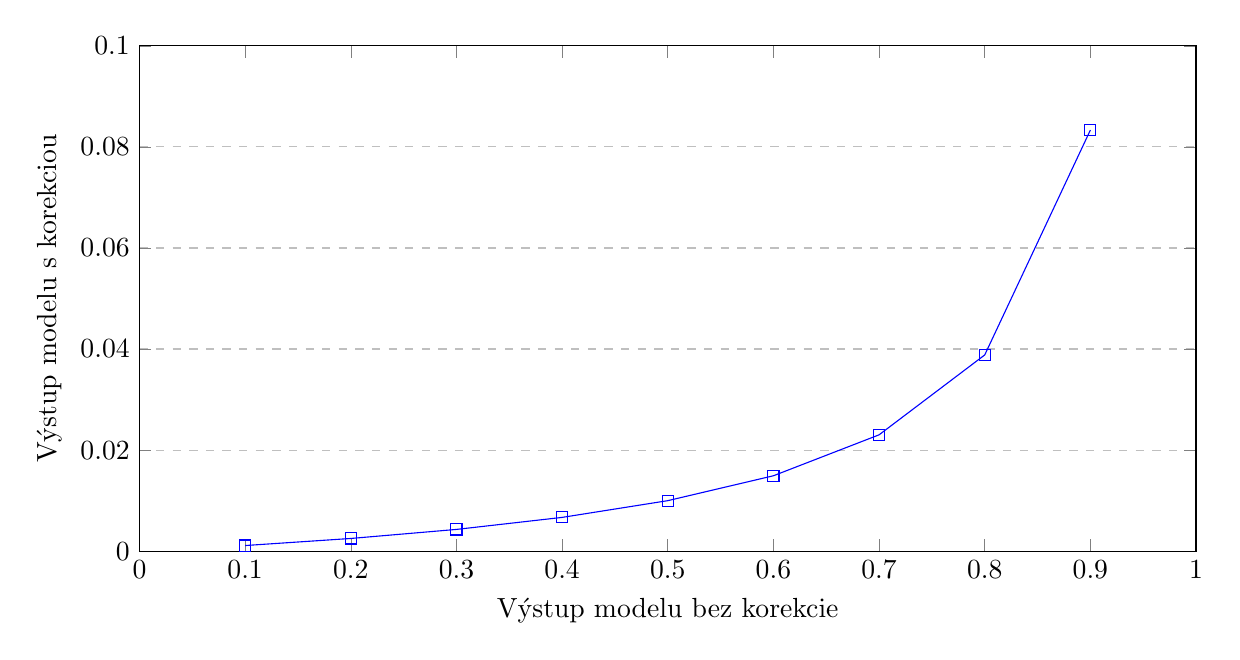
\begin{tikzpicture}
    \begin{axis}[
        xlabel={Výstup modelu bez korekcie},
        ylabel={Výstup modelu s korekciou},
        xmin=0, xmax=1,
        ymin=0, ymax=0.1,
        xtick={0,0.1,0.2,0.3,0.4,0.5,0.6,0.7,0.8,0.9,1},
        ytick={0,0.02,0.04,0.06,0.08,0.1},
        style={
            /pgf/number format/fixed,
            /pgf/number format/precision=3
        },
        legend pos=north west,
        ymajorgrids=true,
        grid style=dashed,
        height=8cm,
        width=15cm,
    ]
    
    \addplot[
        color=blue,
        mark=square,
        ]
        coordinates {
        (0.1, 0.00112107) (0.2, 0.002518892) (0.3, 0.004310345) (0.4, 0.006688963) (0.5, 0.010000000) (0.6, 0.014925373) (0.7, 0.023026316) (0.8, 0.038834951) (0.9, 0.083333333)
        };
        % \legend{Výstup modelu bez korekcie}
    \end{axis}
\end{tikzpicture}
\caption{Graf výstupov logistickej regresie bez korekcie a s korekciou pre skutočnú prevalenciu v populácii \( \pi = 0.01\)}
\label{correction_demo}
\end{figure}

Databáza Finstatu obsahuje od roku 2009 celkovo \(3730\) prípadov bankrotu so známym dátumom začiatku konkurzného alebo reštrukturalizačného konania,
pričom za to isté obdobie obsahuje \(1 403 773\) relevantných záznamov o firmách (jedným záznamom rozumieme pôsobenie firmy počas jedného roka).
Z toho vyplýva prevalencia bankrotu v populácii firiem:

\[
    \pi = \frac{3730}{1403773} \doteq 0.002657125 \doteq 0.266 \%   
\]

a apriórna korekcia:

\[
    \delta = \ln \left[  \frac{1 - \frac{3730}{1403773}}{\frac{3730}{1403773}} \right] \doteq 5.92785
\]

\begin{figure}
    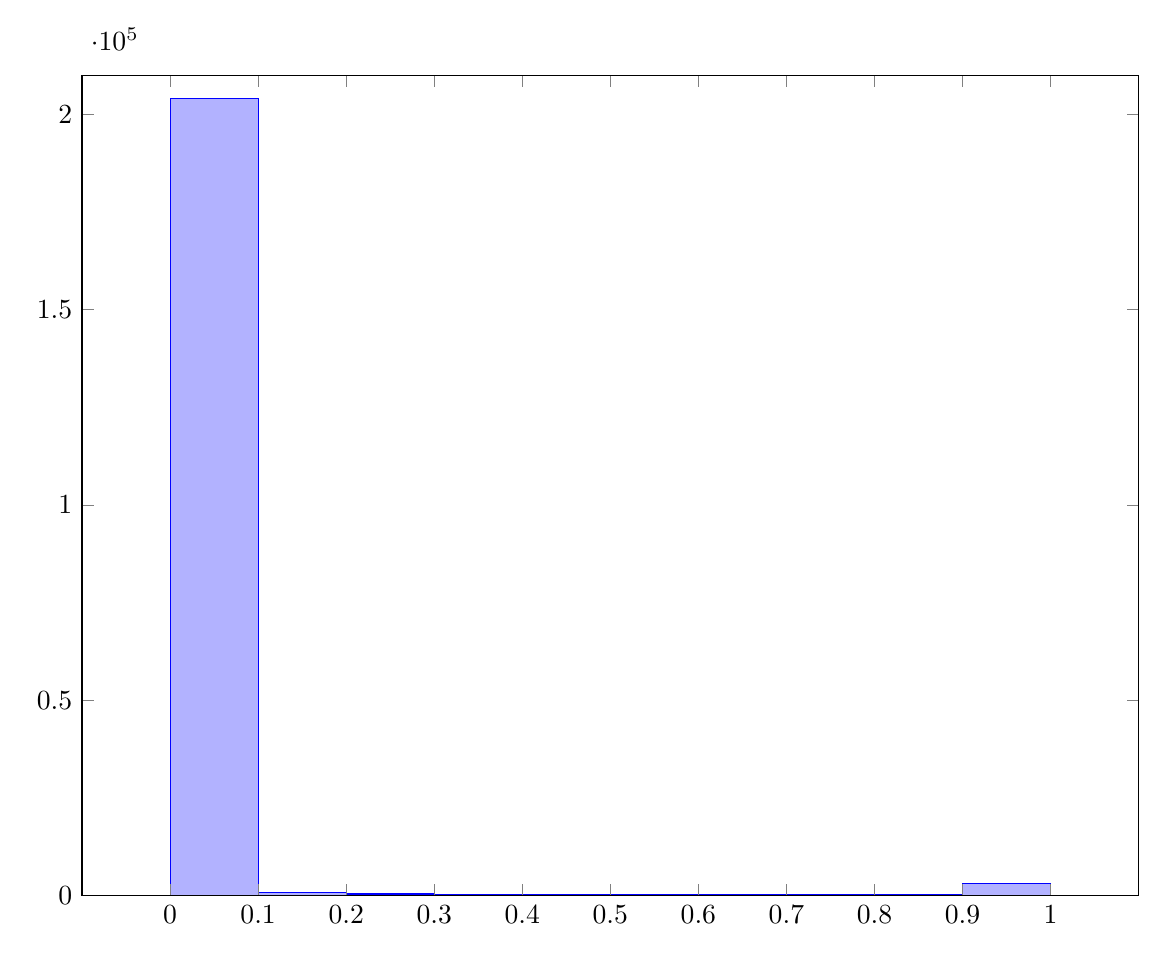
\begin{tikzpicture}
        \begin{axis}[
            ymin=0, ymax=210000,
            % minor y tick num = 2,
            area style,
            xtick={0,0.1,0.2,0.3,0.4,0.5,0.6,0.7,0.8,0.9,1},
            ytick={0,50000,100000,150000,200000},
            style={
                /pgf/number format/fixed,
                /pgf/number format/precision=5
            },
            height=12cm,
            width=15cm,
            ]
        \addplot+[ybar interval,mark=no] plot coordinates {
            (0, 204142) (0.1, 874) (0.2, 440) (0.3, 295) (0.4, 258) (0.5, 258) (0.6, 197) (0.7, 231) (0.8, 333) (0.9, 3195) (1, 0)
        };
        \end{axis}
    \end{tikzpicture}
\caption{Histogram výstupov modelu BACE s apriórnou korekciou pre populáciu \(212169\) slovenských firiem}
\label{model_bace_whole_pop_corrected}
\end{figure}

Obrázok \ref{model_bace_whole_pop_corrected} predstavuje histogram výstupov upraveného BACE modelu, pri znížení interceptu \( \beta_0 \) o hodnotu \( \delta = 5.92785 \).